\documentclass[12pt,a4paper]{report}
\usepackage[margin=1in]{geometry}
\usepackage[T1]{fontenc}
\usepackage{lmodern}
\usepackage{setspace}
\usepackage{booktabs}
\usepackage{longtable}
\usepackage{array}
\usepackage{enumitem}
\usepackage{float}
\usepackage{caption}
\usepackage{subcaption}
\usepackage{tikz}
\usepackage{algorithm}
\usepackage{algpseudocode}
\usepackage[hidelinks]{hyperref}
\usetikzlibrary{arrows.meta,positioning,shapes.geometric,shapes.misc,fit,calc}

\onehalfspacing
\setlist{nosep}
\tikzset{
  block/.style={draw, rounded corners, align=center, font=\scriptsize,
    minimum height=8mm, text width=24mm, fill=blue!5},
  decision/.style={draw, diamond, aspect=2, align=center, font=\scriptsize,
    inner sep=1pt, text width=19mm, fill=yellow!12},
  store/.style={draw, cylinder, shape border rotate=90, aspect=0.25,
    align=center, font=\scriptsize, minimum height=9mm, text width=23mm,
    fill=green!7},
  line/.style={-{Latex[length=2mm]}, thick},
  dashedline/.style={-{Latex[length=2mm]}, dashed, thick}
}

\begin{document}

\chapter{System Design and Methodology}

\section{Overview}
This chapter describes the design and implementation methodology of LabGuard, a
Windows laboratory fleet-management system. The design is based on three
separately deployable projects: a React and TypeScript administrative dashboard,
a FastAPI server, and a Python Windows endpoint agent. The server is the
authority for identity, authorization, validation, durable state and audit
history. Agents collect bounded endpoint observations and perform only typed,
allowlisted operations. The dashboard presents server state and submits
administrator actions; it does not communicate directly with endpoint agents.

The architecture deliberately separates observations from enforcement. For
example, a WFP audit record describes a Windows network decision but is not a
packet capture, while an examination record can report an observed browser or
USB device without blocking it. This distinction is important for both system
correctness and the interpretation of evidence.

\section{System Architecture}

\subsection{Three-tier architecture}
LabGuard follows a three-tier architecture. The presentation layer is the
browser dashboard. It provides fleet, room, telemetry, software, remote
operation, examination, screenshot and camera views. The application layer is
the FastAPI server, which exposes the versioned \texttt{/api/v1} REST contract,
the authenticated agent WebSocket and the administrator SSE invalidation
stream. The data layer consists of PostgreSQL for structured state and
configured file storage for screenshot and camera-evidence images.

\begin{figure}[H]
\centering
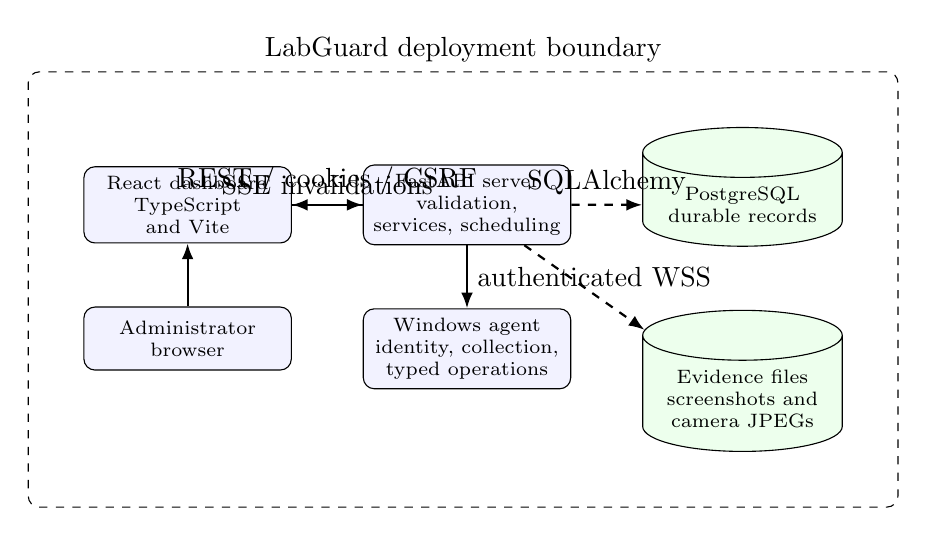
\begin{tikzpicture}[node distance=8mm and 9mm]
\node[block] (dash) {React dashboard\\TypeScript and Vite};
\node[block, right=of dash] (api) {FastAPI server\\validation, services, scheduling};
\node[store, right=of api] (db) {PostgreSQL\\durable records};
\node[store, below=of db] (files) {Evidence files\\screenshots and camera JPEGs};
\node[block, text width=24mm, below=of api] (agent) {Windows agent\\identity, collection, typed operations};
\node[block, below=of dash] (admin) {Administrator browser};
\draw[line] (dash) -- node[above]{REST / cookies / CSRF} (api);
\draw[dashedline] (api) -- node[above]{SQLAlchemy} (db);
\draw[dashedline] (api) -- (files);
\draw[line] (api) -- node[right]{authenticated WSS} (agent);
\draw[line] (api) -- node[above]{SSE invalidations} (dash);
\draw[line] (admin) -- (dash);
\node[draw, dashed, rounded corners, fit=(dash) (api) (db) (files) (agent),
  inner sep=7mm, label=above:{LabGuard deployment boundary}] {};
\end{tikzpicture}
\caption{LabGuard three-tier architecture and communication paths.}
\label{fig:labguard-architecture}
\end{figure}

Figure~\ref{fig:labguard-architecture} shows the principal data paths. Dashboard
requests use same-origin REST and administrator cookies. Mutating requests also
carry the server-issued CSRF token. Agent messages use a separate
ticket-authenticated WebSocket and are never authenticated by a browser
session. The SSE channel contains small invalidation events; the dashboard
refetches canonical records through REST rather than treating SSE as a durable
data store.

\subsection{Component responsibilities and communication}
The dashboard centralizes HTTP calls, renders server responses and provides
forms for authorized actions. It may show or hide controls according to the
administrator role, but server-side role checks remain authoritative.

The server validates Pydantic request and event models, performs role and CSRF
checks, runs domain services, commits state and writes audit records. It also
maintains the agent WebSocket registry, the administrator SSE hub, exam
monitor, screenshot dispatcher and camera sampler. The current scheduler and
event hubs are single-process facilities; a multi-worker deployment would need
shared coordination.

The Windows agent persists its device identity, authenticates to the server,
maintains a heartbeat and executes bounded collectors. It supports telemetry,
software inventory, WFP history, socket snapshots, peripheral observations,
software jobs, process requests, RDP preparation and on-demand screenshots.
It does not expose a general shell or arbitrary command execution.

REST is used for administrator queries and durable mutations. The WebSocket is
used for authenticated, typed device events and request/result exchanges.
Heartbeats, inventory batches and job results are attributed to the device
represented by the authenticated ticket, not to an identifier supplied in a
payload. The database stores metadata, state transitions and bounded histories;
large image bytes are stored outside PostgreSQL with metadata and retention
records in the database.

\subsection{System data flow}
An administrator action follows this sequence:
\begin{enumerate}
\item The browser submits a typed request with the session cookie and CSRF
token.
\item The server checks authentication, role, target state, input bounds and
feature-specific rules.
\item A durable record and its audit event are committed before delivery where
the operation is stateful.
\item If an endpoint action is required, the server sends a fixed event over
the authenticated device socket.
\item The agent validates the event, performs the narrow adapter operation and
sends a typed result or lifecycle event.
\item The server binds the result to the authenticated device and request,
persists it, and publishes an SSE invalidation.
\item The dashboard refetches authoritative state and displays the persisted
result.
\end{enumerate}

\section{Development Methodology}
LabGuard is developed as three projects with explicit boundaries. The server
owns the API contract and database migrations; the client owns Windows-specific
collection and adapter code; and the dashboard owns presentation and typed API
wrappers. Pydantic schemas and typed WebSocket envelopes provide a stable
contract between independently developed components. The envelope contains the
protocol name, schema version, event identifier, device identifier, monotonic
sequence, timestamp, event type and typed payload.

Development is iterative. Features are implemented as a vertical slice:
schema and validation, service and persistence logic, transport event,
endpoint adapter, dashboard query/mutation and focused tests. Alembic
migrations version durable changes. Tests use SQLite where practical for
server logic, while the deployment database is PostgreSQL. Windows-specific
behavior, camera streams and package-manager execution require environment
verification in addition to unit tests. Errors are represented explicitly:
an unavailable manager, incomplete inventory, expired job or failed screenshot
is not converted into a successful empty result.

\section{Requirements Analysis}

\subsection{Functional requirements}
\begin{longtable}{p{0.22\textwidth}p{0.70\textwidth}}
\toprule
\textbf{Area} & \textbf{Requirement}\\
\midrule
Identity & Enroll, approve, reject, enable, disable and revoke endpoint
credentials; maintain administrator sessions and roles.\\
Fleet & Display device status, rooms, positions, liveness, telemetry and
audit history.\\
Collection & Receive heartbeats, telemetry, software inventory, network
history, socket snapshots and peripheral observations.\\
Software & Discover packages, validate exact package identities, create
individual install/uninstall jobs and report verified outcomes.\\
Remote operations & List or terminate a PID-bound process, prepare a
time-limited RDP lease and request an endpoint screenshot.\\
Examinations & Schedule room-based examinations, observe supported signals,
deduplicate violations, collect optional screenshot bursts and produce reports.\\
Physical monitoring & Configure room cameras, sample RTSP streams, run
bounded ONNX detection and retain detection evidence.\\
\bottomrule
\end{longtable}

\subsection{Non-functional, security and operational requirements}
\begin{itemize}
\item \textbf{Reliability:} durable server state, explicit lifecycle states,
acknowledged event delivery and safe reconnection behavior.
\item \textbf{Bounded operation:} payload sizes, batch sizes, process output,
runtime, queues and evidence retention must be bounded.
\item \textbf{Security:} server-managed sessions, RBAC, CSRF protection,
TLS verification, Ed25519 device identity, single-use tickets, input
validation, audit logging and protected file paths.
\item \textbf{Least privilege:} package operations use fixed argument arrays
and \texttt{shell=False}; no endpoint route accepts a shell command, URL or
arbitrary executable path.
\item \textbf{Operational clarity:} offline, expired, uncertain and
incomplete states must be visible rather than inferred as success.
\item \textbf{Deployability:} the agent supports foreground operation and a
Windows service, while the server and dashboard are independently started and
configured.
\end{itemize}

\section{Hardware Requirements}
Deployment requires a server computer, Windows endpoint computers and a local
network connecting administrators and endpoints. The server needs storage for
the PostgreSQL database and configured evidence directories. Endpoint computers
need a supported Windows installation and, for service operation, the
permissions required by the selected machine-level collectors and adapters.

Surveillance cameras require reachable RTSP streams. Camera processing is
CPU-based in the implemented ONNX pipeline, so additional processing capacity
is required when the number of enabled cameras or sampling frequency increases.
No fixed CPU, memory or storage minimum is specified here: capacity depends on
fleet size, telemetry and network-event retention, screenshot frequency,
camera workload and evidence retention. The Windows Security event log also
has finite capacity and its rollover policy affects the recoverable history.

\section{Software Requirements}
\begin{longtable}{p{0.25\textwidth}p{0.65\textwidth}}
\toprule
\textbf{Technology} & \textbf{Role}\\
\midrule
Python 3.12 or later & Server and Windows-agent implementation language.\\
FastAPI and Pydantic & HTTP routing, dependency-based authorization and
typed request/event validation.\\
SQLAlchemy and Alembic & Database mapping, transactions and versioned schema
migrations.\\
PostgreSQL & Intended deployment database for structured durable state.\\
React, TypeScript and Vite & Dashboard component model, type-safe feature
code and development/build tooling.\\
Node.js & Dashboard dependency and build runtime.\\
psutil and pywin32 & Endpoint telemetry, processes, Windows event queries
and operating-system integration.\\
WinGet and Chocolatey & Allowlisted package-manager inventory and operations.\\
OpenCV and ONNX Runtime & Camera frame acquisition, preprocessing and CPU
object inference.\\
\bottomrule
\end{longtable}
The agent also uses Windows DPAPI-protected identity state and Pillow for
bounded screenshot preparation. Exact versions and optional dependencies are
defined in the project manifests; a package being installed on a development
machine does not by itself establish production support.

\section{Database Design}

\subsection{Organization and persistence}
The relational database is organized around authenticated principals, endpoint
state, observations, operations and evidence. Alembic migrations evolve the
schema; the current migration head includes exam management and camera
monitoring records. PostgreSQL is the intended deployment database, while
SQLite is used by selected integration tests. Database transactions group
privileged mutations and their audit records where required.

\begin{figure}[H]
\centering
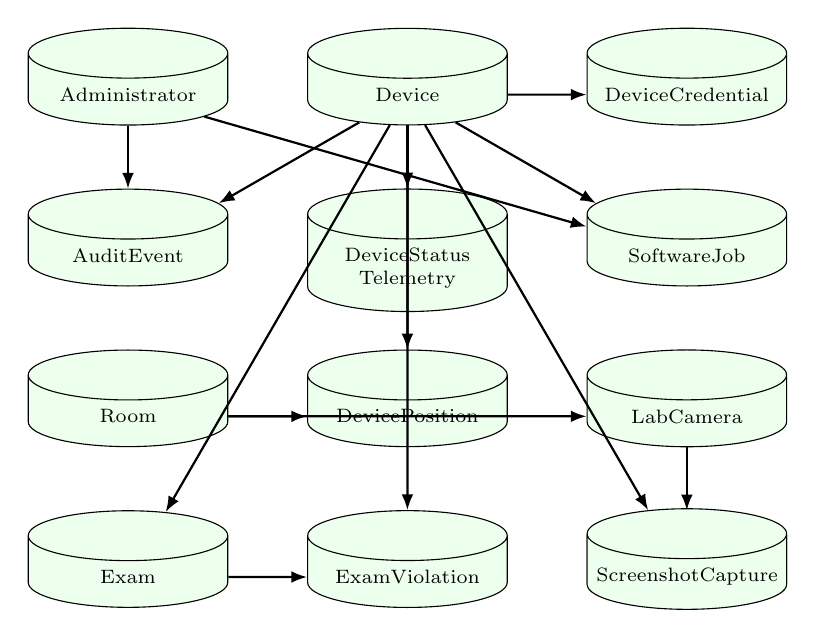
\begin{tikzpicture}[node distance=8mm and 10mm]
\node[store] (admin) {Administrator};
\node[store, right=of admin] (device) {Device};
\node[store, right=of device] (credential) {DeviceCredential};
\node[store, below=of admin] (audit) {AuditEvent};
\node[store, below=of device] (status) {DeviceStatus\\Telemetry};
\node[store, below=of credential] (job) {SoftwareJob};
\node[store, below=of audit] (room) {Room};
\node[store, right=of room] (position) {DevicePosition};
\node[store, right=of position] (camera) {LabCamera};
\node[store, below=of camera] (detection) {CameraDetection};
\node[store, below=of room] (exam) {Exam};
\node[store, right=of exam] (violation) {ExamViolation};
\node[store, right=of violation] (capture) {ScreenshotCapture};
\draw[line] (device) -- (credential);
\draw[line] (device) -- (status);
\draw[line] (device) -- (position);
\draw[line] (room) -- (position);
\draw[line] (room) -- (camera);
\draw[line] (camera) -- (detection);
\draw[line] (device) -- (job);
\draw[line] (device) -- (exam);
\draw[line] (exam) -- (violation);
\draw[line] (device) -- (violation);
\draw[line] (device) -- (capture);
\draw[line] (admin) -- (job);
\draw[line] (admin) -- (audit);
\draw[line] (device) -- (audit);
\end{tikzpicture}
\caption{Main SQLAlchemy entities and foreign-key relationships.}
\label{fig:entity-relationships}
\end{figure}

Figure~\ref{fig:entity-relationships} is a compact view of the relationships
defined in \texttt{models.py}. A device has one credential, one current status
row and many historical telemetry, WFP, peripheral, inventory, job, request
and evidence rows. A room owns device positions and cameras; camera detections
refer to both a camera and its room. An exam stores its target device UUIDs in
JSON and has many deduplicated violations. Administrator foreign keys on jobs,
requests, exams and audit records use nullable or set-null deletion behavior
where defined by the models. Inventory collections and WFP state are omitted
from the figure only to keep the relationship diagram readable; they still
remain device-owned tables with the migration-defined cascade behavior.

Database storage is used for queryable state, timestamps, status transitions,
metadata and retention decisions. Image bytes are file-backed to avoid
inflating relational rows. Screenshot files expire after 24 hours under the
current policy, while camera evidence has its own cleanup service and
metadata-retention settings. File paths are generated and checked against the
configured evidence root.

\section{Device Management}

\subsection{Enrollment and authentication}
An administrator creates a short-lived, one-time enrollment code. The agent
creates or loads a UUID and Ed25519 key pair, protects the private key with
Windows DPAPI, and submits the code, public key and endpoint metadata. The
server stores only a digest of the code, creates a pending device and does not
trust it yet. A LAB\_ADMIN approves or rejects the request. Later, the device
signs a server challenge; after verification the server issues a short-lived,
single-use, device-bound WebSocket ticket. The ticket is stored hashed and is
consumed on connection. Revocation prevents future authentication and closes
an active connection where possible.

\begin{figure}[H]
\centering
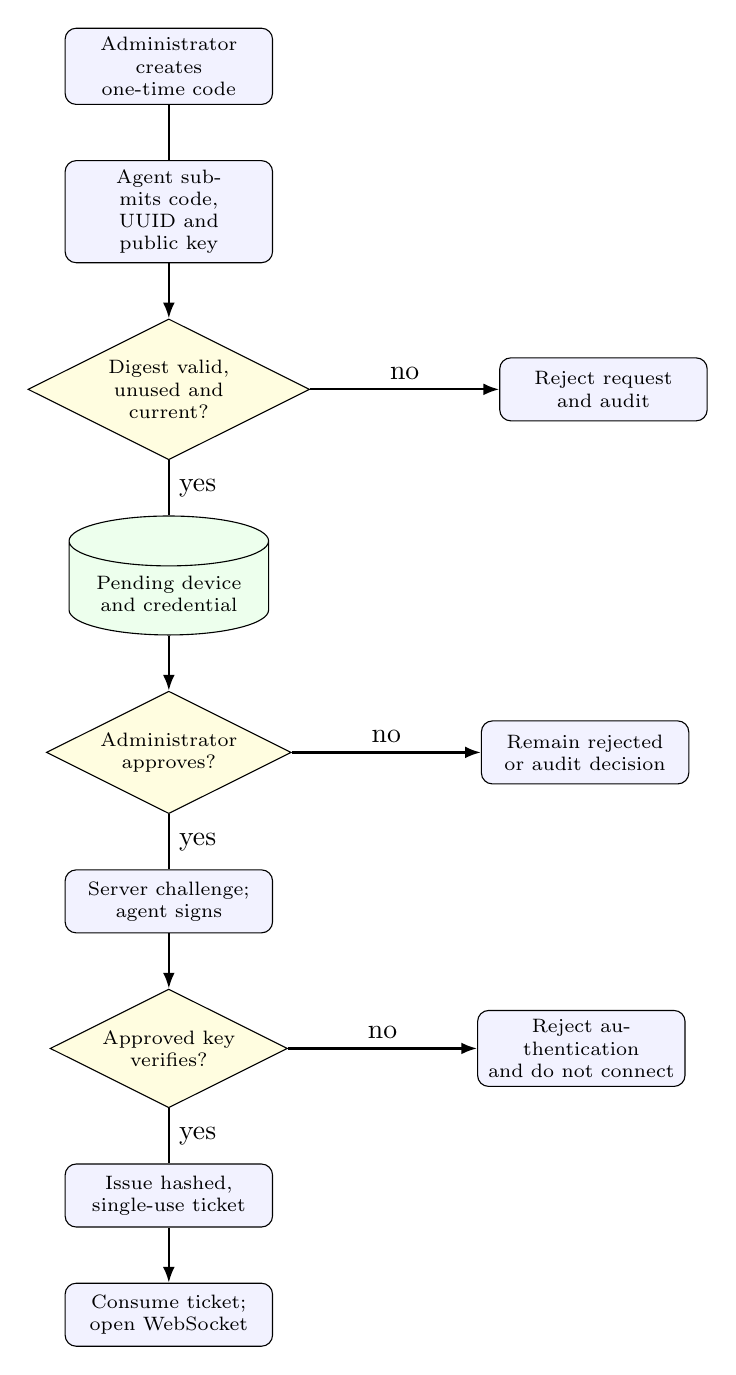
\begin{tikzpicture}[node distance=7mm and 12mm]
\node[block] (code) {Administrator creates\\one-time code};
\node[block, below=of code] (request) {Agent submits code,\\UUID and public key};
\node[decision, below=of request] (valid) {Digest valid,\\unused and current?};
\node[store, below=of valid] (pending) {Pending device\\and credential};
\node[decision, below=of pending] (approve) {Administrator\\approves?};
\node[block, below=of approve] (challenge) {Server challenge;\\agent signs};
\node[decision, below=of challenge] (verify) {Approved key\\verifies?};
\node[block, below=of verify] (ticket) {Issue hashed,\\single-use ticket};
\node[block, below=of ticket] (socket) {Consume ticket;\\open WebSocket};
\node[block, right=of valid, xshift=12mm] (reject-code) {Reject request\\and audit};
\node[block, right=of approve, xshift=12mm] (reject-admin) {Remain rejected\\or audit decision};
\node[block, right=of verify, xshift=12mm] (reject-key) {Reject authentication\\and do not connect};
\draw[line] (code)--(request)--(valid);
\draw[line] (valid)--node[right]{yes}(pending)--(approve);
\draw[line] (valid)--node[above]{no}(reject-code);
\draw[line] (approve)--node[right]{yes}(challenge)--(verify);
\draw[line] (approve)--node[above]{no}(reject-admin);
\draw[line] (verify)--node[right]{yes}(ticket)--(socket);
\draw[line] (verify)--node[above]{no}(reject-key);
\end{tikzpicture}
\caption{Enrollment and authenticated device connection flow.}
\label{fig:device-enrollment-flow}
\end{figure}

Figure~\ref{fig:device-enrollment-flow} shows that possession of an enrollment
code is only a request to enroll. The authenticated socket, rather than a
payload device identifier, supplies the authority used for ingestion.

\begin{algorithm}[H]
\caption{Device enrollment and ticket issuance}
\label{alg:enrollment}
\begin{algorithmic}[1]
\Require enrollment code, public key, device UUID
\State Verify code digest, expiry and unused state
\State Apply enrollment rate limit and validate metadata
\State Consume code and create device in \textsc{Pending} state
\State Await explicit administrator approval
\State Generate random challenge and verify Ed25519 signature
\State Require approved device and non-revoked matching credential
\State Create short-lived ticket, store only its hash, and bind it to device
\State Consume ticket on WebSocket connection
\State Derive device identity from the authenticated connection
\end{algorithmic}
\end{algorithm}

\subsection{Rooms and layout}
An authorized administrator creates a room and submits a complete grid layout.
The server validates device references, coordinate bounds and uniqueness, then
commits the layout atomically. The dashboard renders the room floor plan from
REST state and refetches after SSE invalidation.

\begin{figure}[H]
\centering
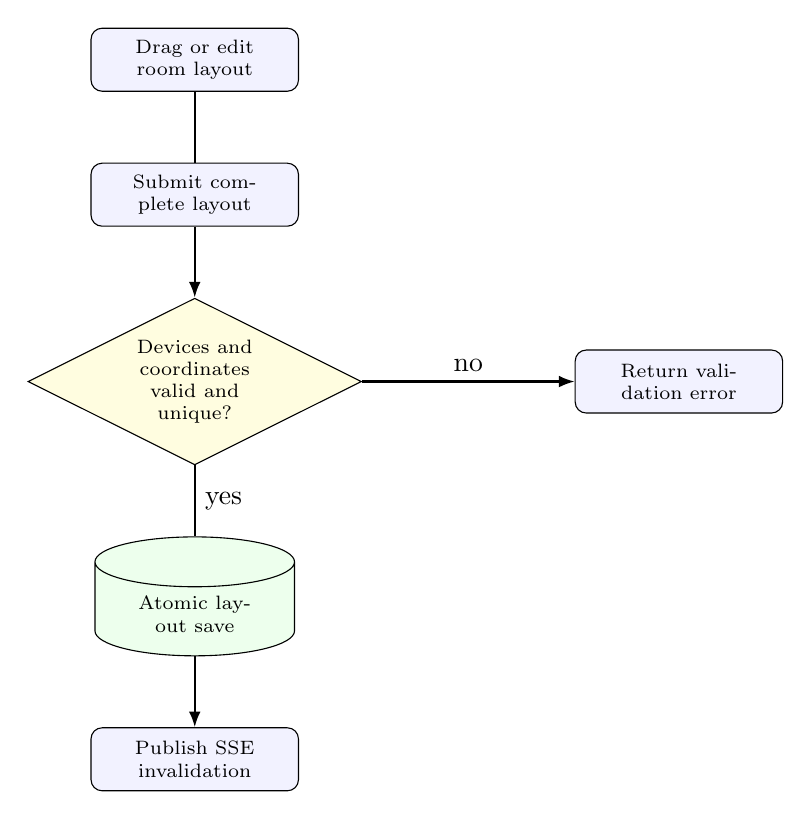
\begin{tikzpicture}[node distance=9mm]
\node[block] (edit) {Drag or edit room layout};
\node[block, below=of edit] (submit) {Submit complete layout};
\node[decision, below=of submit] (check) {Devices and coordinates\\valid and unique?};
\node[store, below=of check] (save) {Atomic layout save};
\node[block, right=of check, xshift=18mm] (error) {Return validation error};
\node[block, below=of save] (notify) {Publish SSE invalidation};
\draw[line] (edit)--(submit)--(check);
\draw[line] (check)--node[right]{yes}(save)--(notify);
\draw[line] (check)--node[above]{no}(error);
\end{tikzpicture}
\caption{Room layout update flow.}
\label{fig:room-layout-flow}
\end{figure}

\section{Device Monitoring and Telemetry}

\subsection{Heartbeat and liveness}
At startup the agent loads protected identity state, authenticates and opens the
socket. It sends periodic heartbeats and reconnects using bounded exponential
backoff with jitter after failures. The server records the time at which an
authenticated heartbeat is received. Liveness is calculated from this server
receipt time, not from an endpoint wall clock. A socket connection alone is not
proof of current heartbeat health.

\begin{figure}[H]
\centering
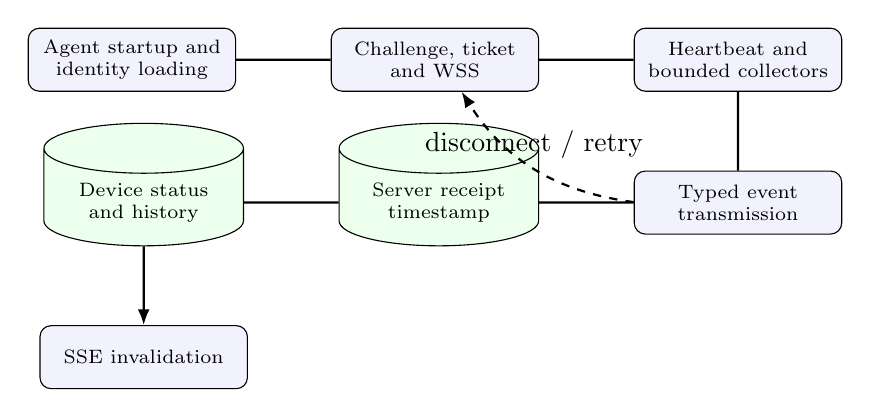
\begin{tikzpicture}[node distance=10mm and 12mm]
\node[block] (start) {Agent startup and\\identity loading};
\node[block, right=of start] (auth) {Challenge, ticket\\and WSS};
\node[block, right=of auth] (collect) {Heartbeat and\\bounded collectors};
\node[block, below=of collect] (send) {Typed event\\transmission};
\node[store, left=of send] (receive) {Server receipt\\timestamp};
\node[store, left=of receive] (status) {Device status\\and history};
\node[block, below=of status] (sse) {SSE invalidation};
\draw[line] (start)--(auth)--(collect)--(send)--(receive)--(status)--(sse);
\draw[dashedline] (send) to[bend left=25] node[above]{disconnect / retry} (auth);
\end{tikzpicture}
\caption{Heartbeat and telemetry pipeline.}
\label{fig:heartbeat-pipeline}
\end{figure}

Figure~\ref{fig:heartbeat-pipeline} distinguishes heartbeat from telemetry.
Heartbeat updates availability. Telemetry describes a machine sample. Software
inventory is a separate, eventually consistent description of installed
software and is not a liveness signal.

\begin{algorithm}[H]
\caption{Authenticated heartbeat processing}
\label{alg:heartbeat}
\begin{algorithmic}[1]
\Require authenticated socket, heartbeat payload
\State Identify device from the ticket-bound connection
\State Validate protocol version, sequence and payload bounds
\State Set \texttt{last\_heartbeat\_at} to current server time
\State Update agent and connection status
\If{status changed}
  \State Record the transition
\EndIf
\State Commit status and publish an admin invalidation
\end{algorithmic}
\end{algorithm}

\subsection{Telemetry and inventory}
The agent collects bounded CPU, memory, disk, host and current-context values,
then sends a typed sample. The server stores server receipt time and exposes
latest and historical views. Collection errors remain distinct from empty
values. Software inventory reads uninstall information from supported registry
views and loaded user hives, and reads local WinGet and Chocolatey listings
when available. It normalizes records, reconciles only unambiguous registry and
WinGet pairs, preserves source provenance and sends bounded batches. The server
replaces the current snapshot only after a complete scan is assembled.

\begin{algorithm}[H]
\caption{Software inventory collection}
\label{alg:inventory}
\begin{algorithmic}[1]
\State Read supported registry uninstall records
\State Run bounded read-only WinGet and Chocolatey list commands
\State Parse and normalize names, versions, publishers, IDs, scope and architecture
\State Reconcile only unique pairs with corroborating identity fields
\State Preserve ambiguous and unmatched records
\State Deduplicate using the source-aware entry key
\State Partition records by count and serialized byte limits
\State Send scan batches and report collection errors separately
\State Replace server snapshot only after all expected batches arrive
\end{algorithmic}
\end{algorithm}

\section{Network and Peripheral Monitoring}

\subsection{WFP events and active sockets}
The agent reads Windows Security events 5156, 5157 and 5152 after installation
enables Filtering Platform Connection auditing. A per-machine cursor and log
generation identify the last acknowledged record. New events enter a bounded
5,000-record queue and are sent in batches of at most 25. The cursor is
persisted only after server acknowledgement. The server validates and
deduplicates on device, log generation and event record ID, and retains event
rows separately from periodic socket snapshots.

\begin{figure}[H]
\centering
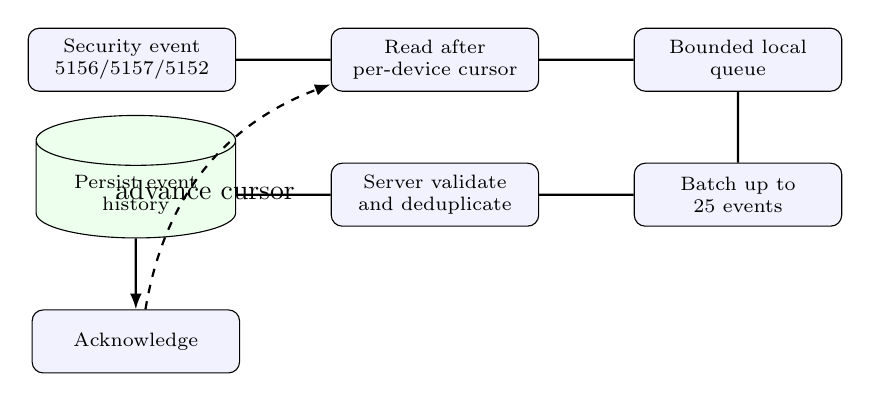
\begin{tikzpicture}[node distance=9mm and 12mm]
\node[block] (event) {Security event\\5156/5157/5152};
\node[block, right=of event] (cursor) {Read after\\per-device cursor};
\node[block, right=of cursor] (queue) {Bounded local\\queue};
\node[block, below=of queue] (batch) {Batch up to\\25 events};
\node[block, left=of batch] (validate) {Server validate\\and deduplicate};
\node[store, left=of validate] (persist) {Persist event\\history};
\node[block, below=of persist] (ack) {Acknowledge};
\draw[line] (event)--(cursor)--(queue)--(batch)--(validate)--(persist)--(ack);
\draw[dashedline] (ack) to[bend left=30] node[below]{advance cursor} (cursor);
\end{tikzpicture}
\caption{WFP event collection and acknowledgement pipeline.}
\label{fig:wfp-pipeline}
\end{figure}

Figure~\ref{fig:wfp-pipeline} shows why acknowledgement is part of the
collection protocol. A disconnect before acknowledgement causes retry rather
than silent cursor advancement. This is event-based audit monitoring, not
packet capture: it does not provide URLs, decrypted HTTPS, credentials or
every UDP, ICMP or short-lived flow.

The agent separately records active TCP and UDP sockets with \texttt{psutil},
normally every 30 seconds. Snapshots can miss short-lived flows and therefore
cannot replace WFP history. Server-side IP enrichment is limited to globally
routable remote addresses. Peripheral observations are also bounded snapshots;
an examination can report an external USB storage observation, but the current
system does not disable that device.

\begin{figure}[H]
\centering
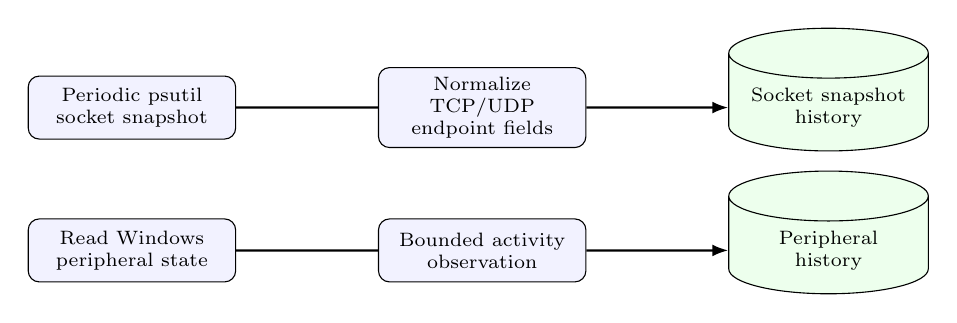
\begin{tikzpicture}[node distance=10mm and 18mm]
\node[block] (snap) {Periodic psutil\\socket snapshot};
\node[block, right=of snap] (normalize) {Normalize TCP/UDP\\endpoint fields};
\node[store, right=of normalize] (socketdb) {Socket snapshot\\history};
\node[block, below=of snap] (usb) {Read Windows\\peripheral state};
\node[block, right=of usb] (per) {Bounded activity\\observation};
\node[store, right=of per] (perdb) {Peripheral\\history};
\draw[line] (snap)--(normalize)--(socketdb);
\draw[line] (usb)--(per)--(perdb);
\end{tikzpicture}
\caption{Independent active-socket and peripheral observation pipelines.}
\label{fig:peripheral-pipeline}
\end{figure}

\section{Software Management}

\subsection{Discovery and inventory}
Server-side WinGet discovery runs bounded \texttt{search --name} and exact
\texttt{show --id} operations using argument arrays and \texttt{shell=False}.
The selected deployable source is the fixed community WinGet source. Search
results are metadata, not approval. Direct installation revalidates the exact
package ID and selected version before creating a job. Chocolatey continues
through its configured catalog/source path.

\begin{figure}[H]
\centering
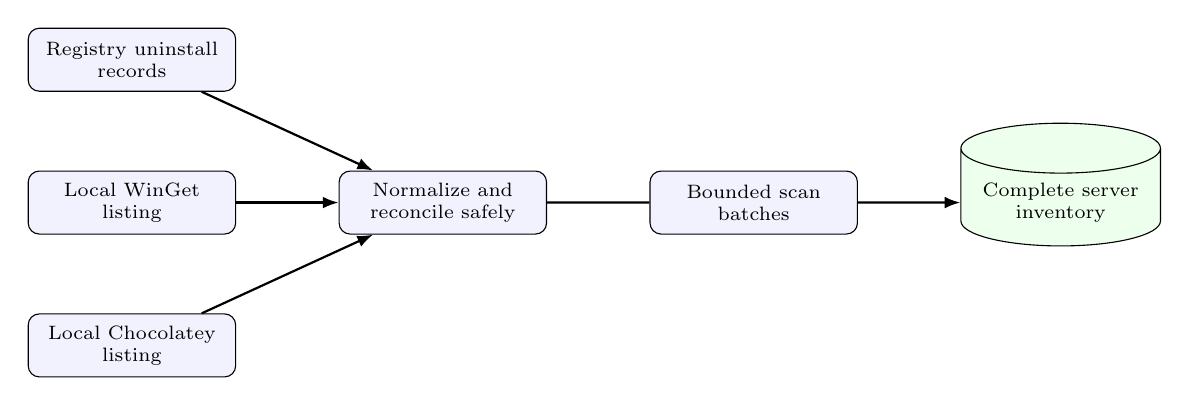
\begin{tikzpicture}[node distance=10mm and 13mm]
\node[block] (reg) {Registry uninstall\\records};
\node[block, below=of reg] (wg) {Local WinGet\\listing};
\node[block, below=of wg] (choco) {Local Chocolatey\\listing};
\node[block, right=of wg] (norm) {Normalize and\\reconcile safely};
\node[block, right=of norm] (batch) {Bounded scan\\batches};
\node[store, right=of batch] (inv) {Complete server\\inventory};
\draw[line] (reg)--(norm);
\draw[line] (wg)--(norm);
\draw[line] (choco)--(norm);
\draw[line] (norm)--(batch)--(inv);
\end{tikzpicture}
\caption{Installed software inventory pipeline.}
\label{fig:software-inventory-flow}
\end{figure}

\subsection{Individual job lifecycle}
The supported operation is a persistent individual job for one device. The
server validates device state, action, manager, exact package identity, scope,
source and repository metadata, writes the job and audit record, and returns
accepted state. Offline jobs remain pending. A connected agent receives a
typed offer, records a durable local journal before side effects, reports
accepted/started/progress/terminal events, executes a constrained adapter and
performs a fresh inventory scan. Success requires verification of the
requested installed or removed state; a manager exit code alone is
insufficient.

\begin{figure}[H]
\centering
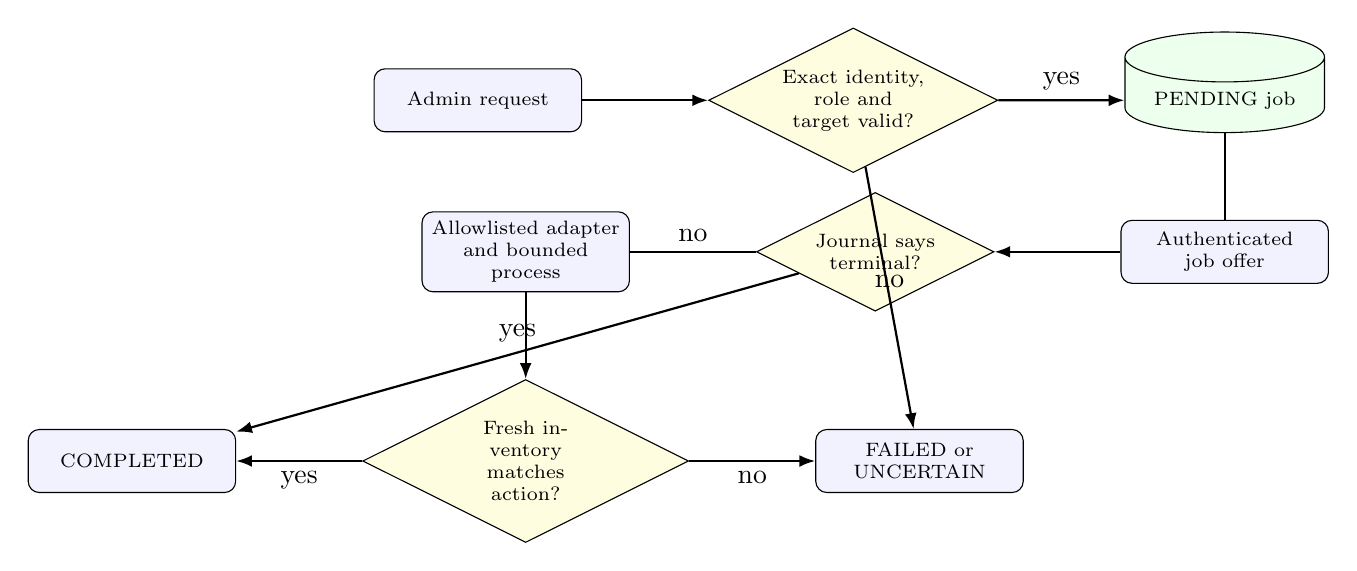
\begin{tikzpicture}[node distance=11mm and 16mm]
\node[block] (request) {Admin request};
\node[decision, right=of request] (valid) {Exact identity,\\role and target valid?};
\node[store, right=of valid] (pending) {PENDING job};
\node[block, below=of pending] (offer) {Authenticated\\job offer};
\node[decision, left=of offer] (journal) {Journal says\\terminal?};
\node[block, left=of journal] (execute) {Allowlisted adapter\\and bounded process};
\node[decision, below=of execute] (verify) {Fresh inventory\\matches action?};
\node[block, left=of verify] (complete) {COMPLETED};
\node[block, right=of verify] (failed) {FAILED or\\UNCERTAIN};
\draw[line] (request)--(valid);
\draw[line] (valid)--node[above]{yes}(pending);
\draw[line] (valid)--node[above]{no}(failed);
\draw[line] (pending)--(offer)--(journal);
\draw[line] (journal)--node[above]{no}(execute)--(verify);
\draw[line] (journal)--node[above]{yes}(complete);
\draw[line] (verify)--node[below]{yes}(complete);
\draw[line] (verify)--node[below]{no}(failed);
\end{tikzpicture}
\caption{Software installation and uninstallation flow.}
\label{fig:software-job-lifecycle}
\end{figure}

\begin{algorithm}[H]
\caption{Validated software job execution}
\label{alg:software-job}
\begin{algorithmic}[1]
\Require typed job offer and authenticated device connection
\State Validate job target, expiry, action, manager, exact ID, scope and source
\State Read durable local journal
\If{terminal result exists}
  \State Replay saved result and stop
\ElsIf{previous execution is uncertain}
  \State Report uncertainty and stop; do not repeat automatically
\EndIf
\State Persist nonterminal journal entry before side effects
\State Execute fixed manager argument array with bounded output and runtime
\State Send lifecycle and progress events
\State Run a complete fresh inventory scan
\If{inventory proves requested state}
  \State Persist and report success
\Else
  \State Persist explicit verification failure
\EndIf
\end{algorithmic}
\end{algorithm}

There is no separate bulk deployment engine and no arbitrary command runner.
Terminal history may be cleared through authorized audited routes, but active
jobs are never deleted.

\section{Remote Administration}

\subsection{Process control and RDP preparation}
Process operations are typed LIST, TERMINATE or KILL requests. A termination
target carries both PID and process creation time, so PID reuse cannot silently
select a different process. Requests expire after 90 seconds and offline
devices fail explicitly.

RDP support prepares access; it does not stream or control a desktop. A
LAB\_ADMIN request is stored and audited, then delivered to an online approved
device. The agent checks Windows edition, elevation and firewall prerequisites,
records original settings, enables the listener and adds request-specific
TCP/3389 rules for a 60-minute lease. Lease expiry, normal shutdown or service
restart restores the saved settings and removes only its own rules. Network
reachability and Windows credentials remain necessary.

\begin{figure}[H]
\centering
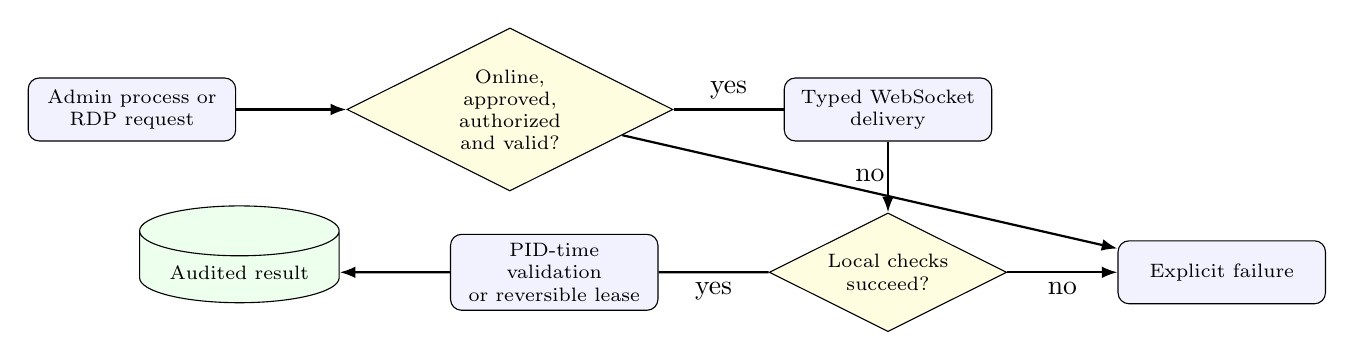
\begin{tikzpicture}[node distance=9mm and 14mm]
\node[block] (op) {Admin process or\\RDP request};
\node[decision, right=of op] (state) {Online, approved,\\authorized and valid?};
\node[block, right=of state] (deliver) {Typed WebSocket\\delivery};
\node[decision, below=of deliver] (local) {Local checks\\succeed?};
\node[block, left=of local] (apply) {PID-time validation\\or reversible lease};
\node[store, left=of apply] (result) {Audited result};
\node[block, right=of local] (fail) {Explicit failure};
\draw[line] (op)--(state);
\draw[line] (state)--node[above]{yes}(deliver)--(local);
\draw[line] (state)--node[above]{no}(fail);
\draw[line] (local)--node[below]{yes}(apply)--(result);
\draw[line] (local)--node[below]{no}(fail);
\end{tikzpicture}
\caption{Remote process operation and RDP preparation pipeline.}
\label{fig:remote-operation-flow}
\end{figure}

\subsection{Screenshot evidence}
An authorized screenshot request is sent over the existing authenticated
socket. Because the service runs in Session 0, it duplicates its token for
the active console session and launches a short-lived noninteractive helper.
The helper creates a downsized JPEG no larger than 1920 by 1080 and 4 MiB.
The service sends sequential 32 KiB chunks. The server validates type, size,
ordering and device association before writing metadata and bytes. Evidence
expires after 24 hours and may be deleted earlier by an authorized
administrator. A screenshot is a momentary screen observation, not proof of
identity or compliance.

\section{Examination Management}

\subsection{Scheduling and monitoring}
An authorized administrator submits timezone-aware start and end times, a room,
desired executable restrictions, browser setting, network mode/CIDR allow-list,
USB setting and evidence option. The server validates time zones, room
membership, CIDRs, supported browser names and overlaps, then persists the
target device set. A same-process monitor changes scheduled records to ACTIVE
and later COMPLETED using UTC time.

\begin{figure}[H]
\centering
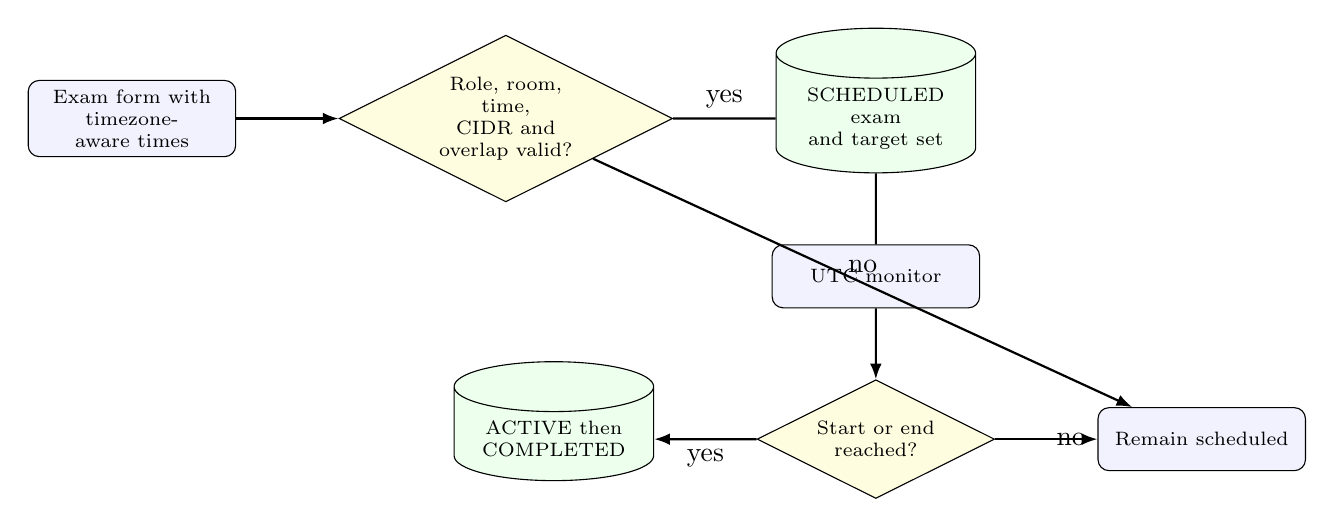
\begin{tikzpicture}[node distance=9mm and 13mm]
\node[block] (form) {Exam form with\\timezone-aware times};
\node[decision, right=of form] (check) {Role, room, time,\\CIDR and overlap valid?};
\node[store, right=of check] (scheduled) {SCHEDULED exam\\and target set};
\node[block, below=of scheduled] (monitor) {UTC monitor};
\node[decision, below=of monitor] (time) {Start or end\\reached?};
\node[store, left=of time] (active) {ACTIVE then\\COMPLETED};
\node[block, right=of time] (wait) {Remain scheduled};
\draw[line] (form)--(check);
\draw[line] (check)--node[above]{yes}(scheduled)--(monitor)--(time);
\draw[line] (check)--node[above]{no}(wait);
\draw[line] (time)--node[below]{yes}(active);
\draw[line] (time)--node[right]{no}(wait);
\end{tikzpicture}
\caption{Examination scheduling and state transition flow.}
\label{fig:exam-scheduling-flow}
\end{figure}

During an active examination, the implemented monitor observes:
\begin{itemize}
\item target devices that are not online, producing an \texttt{AGENT\_OFFLINE}
finding;
\item common browser process-name scans every 15 seconds when enabled,
covering Edge, Chrome and Firefox;
\item allowed WFP connection events outside configured CIDRs when
\texttt{ALLOW\_LIST} is selected; and
\item connected external USB storage when the corresponding observation is
requested.
\end{itemize}
Findings are persisted and deduplicated by examination, device and finding
identity. A browser or other finding can queue four screenshots at detection,
10, 20 and 30 seconds. Missed schedules or disconnected agents fail the
capture records without deleting the violation.

\begin{figure}[H]
\centering
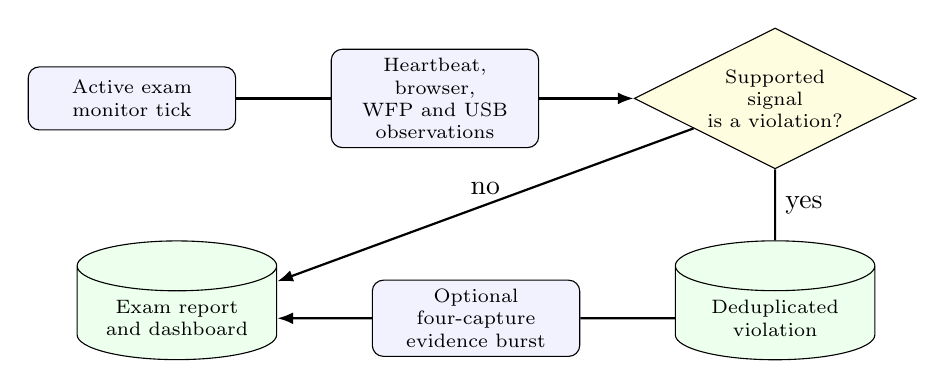
\begin{tikzpicture}[node distance=9mm and 12mm]
\node[block] (activeexam) {Active exam\\monitor tick};
\node[block, right=of activeexam] (signals) {Heartbeat, browser,\\WFP and USB observations};
\node[decision, right=of signals] (finding) {Supported signal\\is a violation?};
\node[store, below=of finding] (record) {Deduplicated\\violation};
\node[block, left=of record] (burst) {Optional four-capture\\evidence burst};
\node[store, left=of burst] (report) {Exam report\\and dashboard};
\draw[line] (activeexam)--(signals)--(finding);
\draw[line] (finding)--node[right]{yes}(record)--(burst)--(report);
\draw[line] (finding)--node[above]{no}(report);
\end{tikzpicture}
\caption{Examination monitoring and violation pipeline.}
\label{fig:exam-monitoring-flow}
\end{figure}

\textbf{Accuracy boundary.} Saved examination restrictions are desired policy
records, not endpoint enforcement policies. The current client does not receive
an examination policy that blocks applications, browsers, USB storage or
network traffic. An allow-list finding is observational; it does not block a
connection. Restricted executable names are stored but are not monitored by
the current described process flow. Reports must therefore distinguish policy
configuration, event observation, violation detection and actual enforcement.

\section{Physical Environment Monitoring}
Camera monitoring is separate from endpoint screenshots. A LAB\_ADMIN creates
a camera under a room with an RTSP URI. The server encrypts the URI with
Fernet and never returns it in ordinary API output. Limits of eight cameras
per room and 32 cameras overall bound the deployment.

\begin{figure}[H]
\centering
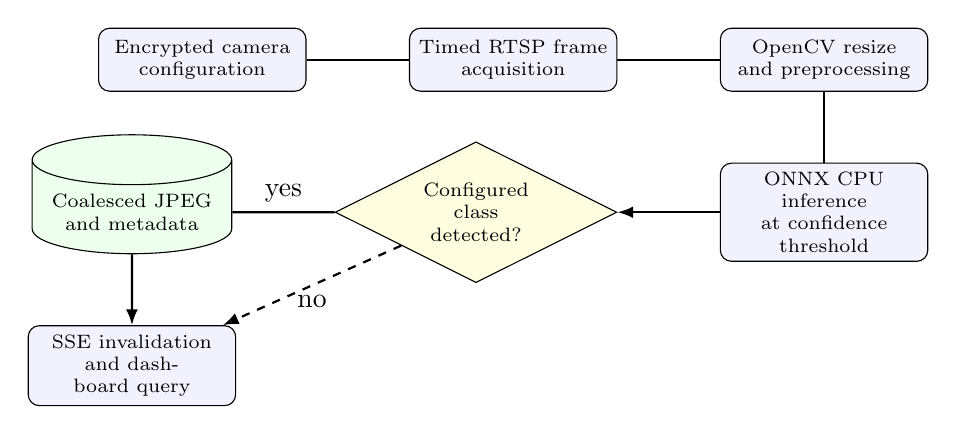
\begin{tikzpicture}[node distance=9mm and 13mm]
\node[block] (config) {Encrypted camera\\configuration};
\node[block, right=of config] (sample) {Timed RTSP frame\\acquisition};
\node[block, right=of sample] (cv) {OpenCV resize\\and preprocessing};
\node[block, below=of cv] (onnx) {ONNX CPU inference\\at confidence threshold};
\node[decision, left=of onnx] (detect) {Configured class\\detected?};
\node[store, left=of detect] (evidence) {Coalesced JPEG\\and metadata};
\node[block, below=of evidence] (dashboard) {SSE invalidation\\and dashboard query};
\draw[line] (config)--(sample)--(cv)--(onnx)--(detect);
\draw[line] (detect)--node[above]{yes}(evidence)--(dashboard);
\draw[dashedline] (detect)--node[below]{no}(dashboard);
\end{tikzpicture}
\caption{Camera sampling and detection-evidence pipeline.}
\label{fig:camera-detection-pipeline}
\end{figure}

Figure~\ref{fig:camera-detection-pipeline} summarizes the asynchronous
pipeline. Sampling and inference run in worker threads. A frame is resized to
300 by 300 for the ONNX model. The current detector accepts configured COCO
food/drink classes at confidence at least 0.40, records counts and maximum
confidence, and writes a reduced annotated JPEG only when an object is
detected. Detections and images are coalesced within a one-minute window to
limit file churn. Evidence expires after 24 hours, and errors clear the
preview while exposing an explicit camera error state.

\begin{algorithm}[H]
\caption{Camera frame processing}
\label{alg:camera}
\begin{algorithmic}[1]
\Require enabled camera with encrypted RTSP URI
\State Decrypt URI in memory and open one bounded RTSP read
\If{open or read fails}
  \State Set explicit camera error and clear preview
\Else
  \State Resize frame and run CPU ONNX inference
  \State Keep only configured classes with confidence at least \(0.40\)
  \If{objects detected}
    \State Draw boxes and encode bounded JPEG preview
    \State Coalesce recent evidence and detection metadata
    \State Persist references and publish dashboard invalidation
  \Else
    \State Update camera state without storing a raw frame
  \EndIf
\EndIf
\end{algorithmic}
\end{algorithm}

Object detection is an indication generated by a model, not definitive proof
of misconduct. Model accuracy, stream compatibility, privacy controls and
capacity must be evaluated in the deployment environment.

\section{Security and Access Control}
Administrator authentication uses server-managed revocable sessions in
HttpOnly cookies. Roles are VIEWER, OPERATOR, LAB\_ADMIN and SUPER\_ADMIN.
Mutations require the session CSRF token in \texttt{X-CSRF-Token}, and role
checks are performed on the server. Device authentication uses an Ed25519
key, challenge response, TLS certificate verification and a short-lived
single-use ticket. Device identity is derived from the ticket-bound socket.

Every privileged mutation is audited with actor, action, target, time and
bounded details. Package execution uses exact package identities, fixed
argument arrays, bounded output/runtime and \texttt{shell=False}. RDP changes
are reversible leases. Screenshot and camera paths are generated, confined
to configured roots and protected by role checks. Camera RTSP URIs are
encrypted at rest. These controls reduce attack surface but do not constitute
a claim that the system is invulnerable; deployment certificates, filesystem
ACLs, credentials and operating-system policy remain operational
responsibilities.

\begin{figure}[H]
\centering
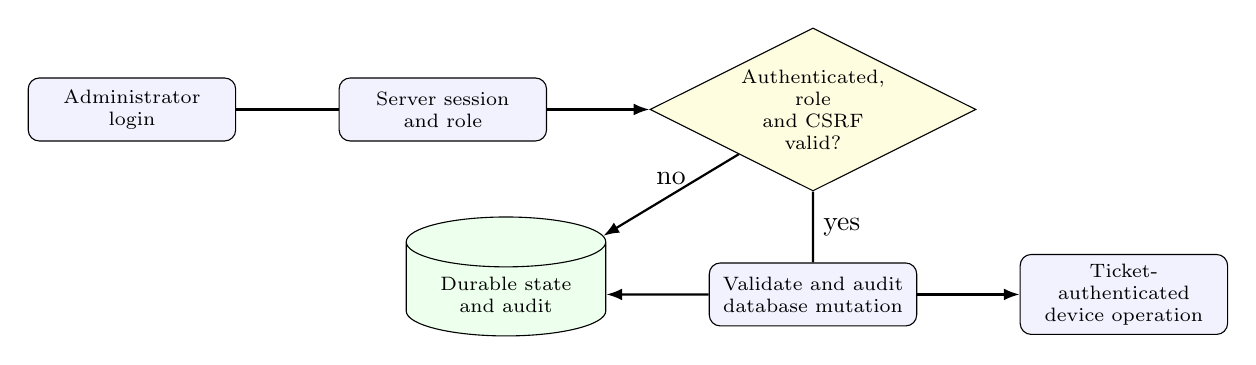
\begin{tikzpicture}[node distance=9mm and 13mm]
\node[block] (login) {Administrator login};
\node[block, right=of login] (session) {Server session\\and role};
\node[decision, right=of session] (authz) {Authenticated, role\\and CSRF valid?};
\node[block, below=of authz] (mutate) {Validate and audit\\database mutation};
\node[block, right=of mutate] (device) {Ticket-authenticated\\device operation};
\node[store, left=of mutate] (records) {Durable state\\and audit};
\draw[line] (login)--(session)--(authz);
\draw[line] (authz)--node[right]{yes}(mutate)--(records);
\draw[line] (authz)--node[above]{no}(records);
\draw[line] (mutate)--(device);
\end{tikzpicture}
\caption{Administrator and device authorization boundary.}
\label{fig:security-flow}
\end{figure}

\section{Error Handling and Data Retention}
Agent disconnections cause heartbeat failure and bounded reconnect attempts.
Invalid WebSocket messages are rejected without allowing a payload to override
connection identity. A failed or expired software job remains visibly failed;
an interrupted running job is uncertain and is not automatically repeated.
Inventory scans distinguish incomplete delivery from a complete empty result.
WFP cursors advance only after acknowledgement, while server deduplication
prevents replayed event rows.

RDP and process requests expire quickly and require online delivery. Screenshot
requests fail when no compatible active console session exists. Camera stream,
model, dependency and storage errors update explicit camera state. Automatic
screenshot evidence is independent from the underlying violation, so a failed
capture does not erase the finding.

Current retention includes 30 days for WFP history, 24 hours for endpoint
screenshot and camera evidence, and feature-specific metadata retention.
Cleanup removes expired files and abandoned partial files while preserving
database consistency. Evidence volume is workload-dependent, especially
because each violation may create four captures. The same-process monitor,
SSE hub, active-device registry and camera sampler are MVP limitations:
multi-worker production deployment requires leader coordination, shared event
fan-out and durable claims to prevent duplicate work.

\section{Chapter Summary}
LabGuard uses a three-tier design in which a server-mediated API and database
separate administrator presentation from endpoint operations. Device
enrollment, cryptographic identity, authenticated WebSocket tickets, server
receipt-time liveness, typed contracts, migrations, audit records and bounded
collectors provide the foundation for safe fleet management. Telemetry,
software inventory, WFP history, socket snapshots and peripheral observations
are intentionally separate data products.

Software operations, process control, RDP preparation and screenshots are
typed, audited and constrained rather than arbitrary remote execution.
Examination scheduling and camera monitoring provide observation and evidence
pipelines, but the current examination restrictions are not endpoint blockers.
This limitation is a core implementation boundary: future enforcement would
require versioned policy delivery, endpoint acknowledgement, reversible
adapters, restart/offline recovery and dedicated validation. The methodology
therefore treats durable state, explicit failure, bounded resource use and
accurate reporting of incomplete functionality as design requirements rather
than optional implementation details.

\end{document}